% Isola o conjunto de elementos pré-textuais com tagging ativo.
\DocumentMetadata{
  lang = pt-BR,
  pdfversion = 1.7,
  pdfstandard = {a-2u, ua-1},
  tagging = on
}
\documentclass[12pt,a4paper,english,brazil]{abntex2}
\usepackage[T1]{fontenc}
\usepackage[utf8]{inputenc}
\usepackage{graphicx}
\usepackage{etoolbox}
\usepackage{hyperref}
\usepackage{amsmath,amssymb,booktabs,tabularx,array}
\usepackage{csvsimple}
\usepackage{listings}
\usepackage[table]{xcolor}
\usepackage[alf]{abntex2cite}
\usepackage{tikz}
\usetikzlibrary{arrows.meta,positioning,shapes.geometric}
\newcommand{\quadroname}{Quadro}
\newfloat[chapter]{quadro}{loq}{\quadroname}
\tagpdfsetup{float/new=quadro}
\renewcommand{\lstlistingname}{Código}
\renewcommand{\lstlistlistingname}{Lista de códigos}
\lstset{
  extendedchars=true,
  literate={á}{{\'{a}}}1 {é}{{\'{e}}}1 {í}{{\'{\i}}}1 {ó}{{\'{o}}}1 {ú}{{\'{u}}}1
    {Á}{{\'{A}}}1 {É}{{\'{E}}}1 {Í}{{\'{I}}}1 {Ó}{{\'{O}}}1 {Ú}{{\'{U}}}1
    {à}{{\`{a}}}1 {À}{{\`{A}}}1 {â}{{\^{a}}}1 {ê}{{\^{e}}}1 {ô}{{\^{o}}}1
    {ã}{{\~{a}}}1 {õ}{{\~{o}}}1 {ç}{{\c{c}}}1 {Ç}{{\c{C}}}1
}
\newcommand{\fontecodigo}[1]{\par\nopagebreak\vspace{2pt}\noindent\textit{\fontename: #1}\par}
\newcommand{\nomealuno}{Nome do aluno}
\newcommand{\cidade}{São Cristóvão/SE}
\newcommand{\anoentrega}{2026}
\newcommand{\dataaprovacao}{dia de mês de 2026}
\newcommand{\titulotrabalho}{Título do trabalho}
\newcommand{\subtitulotrabalho}{}
\newcommand{\nomeorientador}{Nome do professor}
\newcommand{\titulacaoorientador}{Titulação}
\newcommand{\nomecoorientador}{}
\preambulo{Trabalho de Conclusão de Curso.}
\begin{document}
\selectlanguage{brazil}
\begin{capa}
  \begin{center}
    \begin{minipage}{0.14\textwidth}\centering
\includegraphics[height=1.55cm,alt={Brasão da Universidade Federal de Sergipe}]{figuras/logo-ufs.pdf}\end{minipage}%
    \begin{minipage}{0.72\textwidth}\centering\small
      UNIVERSIDADE FEDERAL DE SERGIPE\\
      CENTRO DE CIÊNCIAS EXATAS E TECNOLOGIA\\
      DEPARTAMENTO DE ENGENHARIA DE PRODUÇÃO
    \end{minipage}%
    \begin{minipage}{0.14\textwidth}\centering
\includegraphics[height=1.55cm,alt={Logotipo do Departamento de Engenharia de Produção da UFS}]{figuras/logo-depro.pdf}\end{minipage}

    \vspace*{3.4cm}
    {\normalsize\MakeUppercase{\nomealuno}\par}
    \vfill
    {\SingleSpacing\bfseries\MakeUppercase{\titulotrabalho}\ifdefempty{\subtitulotrabalho}{}{: \normalfont\subtitulotrabalho}\par}
    \vfill\vfill
    {\cidade\par}
    {\anoentrega\par}
  \end{center}
\end{capa}

% Não utilizar titlingpage aqui para preservar a contagem sequencial a partir
% da folha de rosto, conforme a ABNT NBR 14724 (seção 5.3).
\thispagestyle{empty}
\pdfbookmark[0]{Folha de rosto}{folha-de-rosto}
\begin{center}
  \MakeUppercase{\nomealuno}\par
  \vspace*{3cm}
  {\SingleSpacing\bfseries\MakeUppercase{\titulotrabalho}\ifdefempty{\subtitulotrabalho}{}{: \normalfont\subtitulotrabalho}\par}
  \vspace*{3cm}
\end{center}
\noindent\hspace*{0.5\textwidth}\begin{minipage}{0.5\textwidth}\SingleSpacing\small
  \imprimirpreambulo
  \par\vspace{0.7cm}
  Orientador: \nomeorientador % Altere para Orientadora: / Coorientadora: quando aplicável
  \ifdefempty{\nomecoorientador}{}{\\Coorientador: \nomecoorientador}
\end{minipage}
\vfill
\begin{center}\cidade\\\anoentrega\end{center}
\cleardoublepage

\begin{folhadeaprovacao}
  \begin{center}
    \MakeUppercase{\nomealuno}\par
    \vspace*{1cm}
    {\SingleSpacing\bfseries\MakeUppercase{\titulotrabalho}\ifdefempty{\subtitulotrabalho}{}{: \normalfont\subtitulotrabalho}\par}
    \vspace*{1.7cm}
  \end{center}
  Este documento foi julgado adequado como requisito parcial à obtenção do título de bacharel em Engenharia de Produção pela Universidade Federal de Sergipe e aprovado em sua forma final.
  \begin{center}\vspace{0.8cm}\cidade, \dataaprovacao\end{center}
  \vspace{0.8cm}\noindent BANCA EXAMINADORA:
  \begin{center}
    \vspace*{1.1cm}\rule{8cm}{0.4pt}\\
    \nomeorientador, \titulacaoorientador\\Universidade Federal de Sergipe
    \ifdefempty{\nomecoorientador}{}{%
      \par\vspace*{1.1cm}\rule{8cm}{0.4pt}\\
      \nomecoorientador, Titulação\\Instituição%
    }
    \par\vspace*{1.1cm}\rule{8cm}{0.4pt}\\
    Nome do Membro, Titulação\\Instituição
    \par\vspace*{1.1cm}\rule{8cm}{0.4pt}\\
    Nome do Membro, Titulação\\Instituição
  \end{center}
\end{folhadeaprovacao}

\begin{agradecimentos}
  Agradecimentos.
\end{agradecimentos}

\begin{resumo}
  \noindent Escreva aqui o resumo do trabalho em parágrafo único, apresentando objetivo, metodologia, resultados principais e conclusão, com extensão recomendada de 150 a 500 palavras conforme a ABNT NBR 6028. Substitua este texto pelo conteúdo definitivo.

  \vspace{\onelineskip}
  \noindent\textbf{Palavras-chave:} primeiro termo; segundo termo; terceiro termo.
\end{resumo}

\begin{abstract}
  \begin{center}
    \ABNTEXchapterfont\ABNTEXchapterfontsize\bfseries\MakeUppercase{Abstract}
  \end{center}
  \begin{otherlanguage*}{english}
    \noindent Write the abstract here in a single paragraph, covering the objective, method, main findings, and conclusion (150 to 500 words according to ABNT NBR 6028). Replace this text with your final content.

    \vspace{\onelineskip}
    \noindent\textbf{Keywords:} first keyword; second keyword; third keyword.
  \end{otherlanguage*}
\end{abstract}

\chapter{Capítulo de teste}
Este parágrafo verifica o texto corrido após os elementos pré-textuais.
\chapter{Introdução}
Apresente aqui o contexto, o problema de pesquisa, a justificativa e a organização do trabalho. As diretrizes gerais de estrutura e apresentação de trabalhos acadêmicos estão definidas na norma vigente \cite{abnt14724}; um exemplo de citação no texto pode ser feito com \citeonline{gil2022}.

A Figura~\ref{fig:exemplo} ilustra a inserção de uma figura baseada no modelo institucional~\cite{depro2021}, o Quadro~\ref{qua:exemplo} exemplifica um quadro editável (fechado nas quatro laterais, voltado a dados qualitativos) e a Tabela~\ref{tab:exemplo} demonstra uma tabela numérica no padrão tabular aberto.

\begin{figure}[htbp]
  \centering
  \caption{Título da figura}\label{fig:exemplo}
  
\includegraphics[height=1.8cm,alt={Logotipo do Departamento de Engenharia de Produção da UFS utilizado como figura de exemplo}]{figuras/logo-depro.pdf}
  \fonte{\citeonline{depro2021}}
\end{figure}

\begin{quadro}[htbp]
  \centering
  \caption{Título do quadro}\label{qua:exemplo}
  \tagpdfsetup{table/header-rows={1}}
  \begin{tabularx}{\textwidth}{|>{\bfseries\raggedright\arraybackslash}p{3.8cm}|>{\raggedright\arraybackslash}X|>{\raggedright\arraybackslash}X|}
    \hline
    \rowcolor{gray!12}
    \textbf{Coluna A} & \textbf{Coluna B} & \textbf{Coluna C} \\ \hline
    Exemplo & Texto editável & Resultado \\ \hline
    Outro exemplo & Texto editável & Resultado \\ \hline
  \end{tabularx}
  \fonte{Elaboração própria}
\end{quadro}

\begin{table}[htbp]
  \centering
  \caption{Título da tabela}\label{tab:exemplo}
  \tagpdfsetup{table/header-rows={1}}
  \begin{tabular}{lrrr}
    \toprule
    \textbf{Item} & \textbf{Quantidade (unid.)} & \textbf{Área ($\text{m}^2$)} & \textbf{Custo (R\$)} \\
    \midrule
    A & 6.529 & 9.482 & 647 \\
    B & 4.894 & 6.524 & 644 \\
    C & 556 & 5.675 & 238 \\
    D & 2.546 & 649 & 787 \\
    \midrule
    \textbf{Total} & \textbf{14.525} & \textbf{22.330} & \textbf{2.316} \\
    \bottomrule
  \end{tabular}
  \fonte{Elaboração própria}
\end{table}

Um exemplo de equação numerada e referenciada como Equação~\eqref{eq:area} é dado por:
\begin{equation}\label{eq:area}
  A = \pi r^2
\end{equation}
\needspace{4\baselineskip}
\noindent em que:
\par\nopagebreak\vspace{0.3em}\nopagebreak
\begin{description}
  \item[$A$] área de um círculo, medida em $[\text{m}^2]$;
  \item[$r$] raio da circunferência.
\end{description}

\chapter{Objetivos}

\section{Objetivo geral}
O trabalho tem como objetivo geral [...].

\section{Objetivos específicos}
Para atingir o objetivo geral, foram delineados os seguintes objetivos específicos:
\begin{alineas}
  \item objetivo específico 1;
  \item objetivo específico 2;
  \item objetivo específico 3.
\end{alineas}

\chapter{Revisão da literatura}
Desenvolva aqui a fundamentação teórica com citações diretas e indiretas no padrão autor-data \cite{abnt10520}. Trabalhos de referência podem ser citados no corpo da frase, como \citeonline{gil2022}, ou entre parênteses ao final da oração \cite{slack2018}. Fontes eletrônicas disponíveis na internet também podem ser referenciadas normalmente no texto \cite{abntex2site}.

Para citações diretas com mais de três linhas, utilize o ambiente \texttt{citacao}, que aplica automaticamente o recuo de 4~cm da margem esquerda, fonte reduzida e espaçamento simples, dispensando aspas e exigindo a indicação da página conforme a \citeonline{abnt10520}:

\begin{citacao}
Exemplo de citação direta longa transcrita literalmente da obra consultada, redigida com extensão suficiente para ultrapassar três linhas na formatação final do documento, demonstrando o recuo de 4~cm, a fonte menor e o espaçamento simples entre linhas exigidos pelas normas vigentes \cite[p.~15]{gil2022}.
\end{citacao}

\chapter{Procedimentos metodológicos}
Descreva o enquadramento metodológico da pesquisa~\cite{gil2022}, o objeto de estudo, os instrumentos de coleta de dados e as etapas de análise. A Figura~\ref{fig:roteiro} apresenta um exemplo editável de roteiro metodológico desenhado diretamente em TikZ (fluxo sequencial composto por coleta de dados, etapas 1 a 4 e análise dos resultados).

\begin{figure}[htbp]
  \centering
  \caption{Roteiro de trabalho}\label{fig:roteiro}
  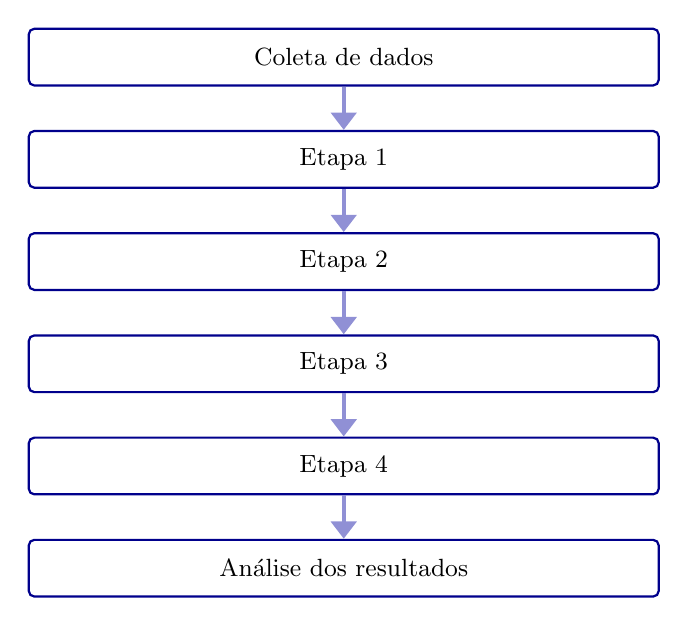
\begin{tikzpicture}[
    node distance=0.55cm,
    etapa/.style={
      rectangle,
      rounded corners=2pt,
      draw=blue!55!black,
      line width=0.8pt,
      minimum width=8cm,
      text width=7.2cm,
      minimum height=0.72cm,
      align=center,
      font=\small
    },
    seta/.style={
      -{Triangle[length=2.2mm,width=3.2mm]},
      draw=blue!45!gray!60,
      line width=1.6pt
    }
  ]
    \node[etapa] (e0) {Coleta de dados};
    \node[etapa, below=of e0] (e1) {Etapa 1};
    \node[etapa, below=of e1] (e2) {Etapa 2};
    \node[etapa, below=of e2] (e3) {Etapa 3};
    \node[etapa, below=of e3] (e4) {Etapa 4};
    \node[etapa, below=of e4] (e5) {Análise dos resultados};

    \draw[seta] (e0) -- (e1);
    \draw[seta] (e1) -- (e2);
    \draw[seta] (e2) -- (e3);
    \draw[seta] (e3) -- (e4);
    \draw[seta] (e4) -- (e5);
  \end{tikzpicture}
  \fonte{Elaboração própria}
\end{figure}

\noindent\textbf{Descrição do roteiro:} o processo segue em sequência, da coleta de dados às etapas 1, 2, 3 e 4, e termina na análise dos resultados.

\chapter{Resultados e discussão}
Apresente os resultados obtidos e discuta seu significado à luz da literatura revisada. A Tabela~\ref{tab:exemplo-csv} demonstra como importar dados diretamente de um arquivo CSV externo utilizando o pacote \texttt{csvsimple}.

% ATENÇÃO: o arquivo CSV deve estar previamente tratado e pronto para exibição
% (casas decimais arredondadas, separador decimal com vírgula no padrão
% brasileiro, separador de colunas ";" e eventuais totais já calculados).
% O LaTeX apenas lê e formata a tabela visualmente, sem processar dados brutos.
\begin{table}[htbp]
  \centering
  \caption{Desempenho operacional importado de arquivo CSV}\label{tab:exemplo-csv}
  \tagpdfsetup{table/header-rows={1}}
  \csvreader[
    separator=semicolon,
    respect all,
    tabular=lrrr,
    table head=\toprule \textbf{Linha} & \textbf{Tempo de ciclo (min)} & \textbf{Eficiência (\%)} & \textbf{Produção diária (unid.)} \\ \midrule,
    late after line=\\,
    table foot=\bottomrule
  ]{dados/exemplo-tabela.csv}{}{%
    \csvcoli & \csvcolii & \csvcoliii & \csvcoliv
  }
  \fonte{Elaboração própria}
\end{table}

\chapter{Considerações finais}
Retome os objetivos do trabalho, sintetize as principais conclusões, registre as limitações da pesquisa e sugira recomendações para trabalhos futuros.

\postextual
% Apêndices contêm material elaborado pelo próprio autor.
% Caso deseje página divisória própria, descomente \partapendices.
\begin{apendicesenv}
  % \partapendices
  \chapter{Título do apêndice}
  Inclua aqui o material produzido pelo autor que complementa o trabalho (questionários, códigos-fonte, deduções extensas, entre outros).

% --------------------------------------------------------------------------
% Exemplo opcional de inserção de códigos-fonte (pacote listings)
% Linguagens prontas para uso: Python, R, SQL, Matlab e VBA.
% Acentos UTF-8 em português são suportados diretamente nos comentários e
% strings. Caso utilize códigos-fonte no TCC, lembre-se de descomentar
% \tagstructbegin{tag=TOC}
\listofcodigos*
\tagstructend
\cleardoublepage
 em tcc-depro-ufs.tex.
% --------------------------------------------------------------------------
%
% 1) Código escrito diretamente no arquivo .tex:
%
% \begin{lstlisting}[
%   language=Python,
%   caption={Cálculo de indicador de eficiência operacional},
%   label={cod:exemplo-python}
% ]
% # Cálculo da eficiência média com comentários em UTF-8 (ação, produção)
% def calcular_eficiencia(producao_real, capacidade_nominal):
%     if capacidade_nominal <= 0:
%         raise ValueError("Capacidade deve ser maior que zero.")
%     return (producao_real / capacidade_nominal) * 100.0
%
% print(f"Eficiência: {calcular_eficiencia(420, 500):.1f}%")
% \end{lstlisting}
% \fontecodigo{Elaboração própria}
%
% 2) Importação de arquivo externo (ex.: Python, R, SQL, Matlab ou VBA):
%
% \lstinputlisting[
%   language=VBA,
%   caption={Rotina de otimização no Excel Solver via macro VBA},
%   label={cod:exemplo-vba}
% ]{dados/macro-solver.bas}
% \fontecodigo{Elaboração própria}
\end{apendicesenv}

\end{document}
